\section{Numerical experiments}\label{sec:numerics}

The computations have three purposes: to confirm the rates and constants of the theorems, to separate the leak from the geometric error, and to carry out the study of the penalty that Scott's question asks for. We report a selection; the full study, with all tables, is in \cite{PadhiExt}, and all code, raw outputs and logs are in the public repository \cite{ZeroGradRepo}.

\subsection{Setup}
Except where stated we use $P_4$ Scott--Vogelius elements (all ten $P_3$ divergence moments per triangle), Nitsche's method on the inscribed polygon, and strong Dirichlet data on the square $R=(-2.5,2.5)^2$. The vertices of $\Gh$ are the radial projections of $N$ equispaced points on the square, so the chords are not all equal ($\max|e|/\min|e|$ grows from $1.43$ at $N=16$ to $1.97$ at $N=256$). The ratio $h/\hG$ stays in $3.28$--$3.48$, so rates in $h$ and $\hG$ coincide; $h$ decreases from $1.505$ ($N=16$) to $0.109$ ($N=256$). Rates in the tables are computed between consecutive runs of the full sequence $N=16,24,32,48,64,96,128,192,256$, some of which are omitted from the tables. Every polygon vertex lies in three triangles (mesh (s)), except on the alternating mesh (a) of Section~\ref{sec:num:strong}. Saddle-point systems are solved by SuperLU \cite{SuperLU} with iterative refinement; over the $148$ production solves the relative residual is at most $3.8\cdot10^{-15}$ and the discrete divergence at most $7\cdot10^{-11}$. As a cross-check, for the constant-pressure benchmark of \cite{Cavalcante} our code gives the coercivity threshold $\mu^\ast=60.343$ at $N=20$, against the transition $60.33821<\mu^\ast<60.33831$ reported there.

The test problems are:
\begin{itemize}
\item[\textbf{A}] Scott's benchmark, the rotating shear flow $u=(1-r^{-2})(-y,x)$ with $p\equiv0$, so $G=0$;
\item[\textbf{B$_a$}] $\psi=(r^2-1)^2(x+y^2/2)/10$ and $p=a(x^2y-y+x/2)$, so $G=a(7\pi/8)^{1/2}$ ($1.658$ for $a=1$, $165.8$ for $a=100$);
\item[\textbf{P}] pure pressure: $u\equiv0$, $f=\nabla p$ with $p$ as in B$_1$. $\CNS$ reproduces this exactly, so the $\GS$ output is \emph{exactly} the response to the missing traction;
\item[\textbf{C}] $\psi$ as in B with the non-polynomial pressure $p=e^{x/2}\cos y$.
\end{itemize}
The manufactured solutions are smooth on the whole box, so the corner caveat of Assumption~\ref{ass:D} does not arise.

\emph{The production penalty.} Most runs use $\mu=100$, i.e.\ $\gamma\approx29$--$30$. This is only $1.37$--$1.41$ times the measured coercivity threshold of $\GS$ on $\Zh$. For $\CNS$ the relevant quantity is the largest $\mu$ at which the square system is singular: $\mu_c=78.9$, $84.4$, $88.1$ at $N=16$, $32$, $64$, extrapolating to about $93$. \begin{center}\small
\setlength{\tabcolsep}{3pt}\begin{tabular}{rccc}
\toprule
$N$ & $\mu^\ast$ ($\GS$ coercivity) & $\mu_c$ ($\CNS$ singular) & margin of $\mu=100$ for $\CNS$\\
\midrule
16 & 59.3 & 78.9 & 27\%\\
32 & 66.0 & 84.4 & 19\%\\
64 & 70.7 & 88.1 & 13\%\\
$\infty$ (extrapolated) & $\approx73$ & $\approx93$ & $\approx7\%$\\
\bottomrule
\end{tabular}
\end{center}
So $\mu=100$ is stable for $\CNS$ on every production mesh, but the margin shrinks from $27\%$ ($N=16$) to $13\%$ ($N=64$), and to about $7\%$ in the limit. The thresholds $\gamma_0,\gamma_2$ of the proofs are not computed, so these runs illustrate the theorems rather than being covered by them. Near the threshold the discrete solution is amplified by a factor of order $(1-\mu^\ast/\mu)^{-1}$, which drifts from about $2.5$ to $3.4$ over $N=16\to64$ and can lower measured rates by up to about $0.2$ per doubling at $N\le64$; normalised constants at $\mu=100$ are partly pre-asymptotic, and we quote larger penalties alongside where we have them.

\subsection{Scott's rate for the corrected method}
Table~\ref{tab:cns} shows the $H^1$ errors of $\CNS$. The rates decrease monotonically towards $\frac32$, the geometric term, for both tests; at $N=256$ the energy rate is $1.52$ and the slip rate $2.02$ (the slip carries an extra factor $(h/\mu)^{1/2}$). The term $h^4$ is invisible at these levels. The error does not depend on the pressure: for polynomial pressures this is structural ($p\in\Pih$), and B$_1$ and B$_{100}$ agree to all printed digits; with the non-polynomial pressure of test C the $H^1$ error differs from that of B$_1$ by a relative $7.9\cdot10^{-7}$, $3.9\cdot10^{-8}$ and $9.7\cdot10^{-9}$ at $N=16$, $64$ and $96$, the size of the higher-order projection term. For $k=5$ and $6$ the $\CNS$ rates on B$_1$ are $1.58$--$1.61$ at the finest levels, non-increasing, with nearly equal errors for $k=4,5,6$: the geometric term dominates.

\begin{table}[t]
\centering\small
\caption{$\CNS$ attains Scott's rate $\hG^{3/2}$: $H^1$ error, $k=4$, $\mu=100$.}\label{tab:cns}
\begin{tabular}{rrcccc}
\toprule
$N$ & $h$ & A & rate & B$_1$ & rate\\
\midrule
32 & 0.813 & $6.41\cdot10^{-2}$ & 1.80 & $2.34\cdot10^{-2}$ & 2.43\\
64 & 0.422 & $2.08\cdot10^{-2}$ & 1.69 & $6.83\cdot10^{-3}$ & 1.76\\
96 & 0.285 & $1.09\cdot10^{-2}$ & 1.64 & $3.54\cdot10^{-3}$ & 1.68\\
128 & 0.215 & $6.96\cdot10^{-3}$ & 1.60 & $2.24\cdot10^{-3}$ & 1.63\\
192 & 0.144 & $3.71\cdot10^{-3}$ & 1.58 & $1.19\cdot10^{-3}$ & 1.60\\
256 & 0.109 & $2.39\cdot10^{-3}$ & 1.56 & $7.58\cdot10^{-4}$ & 1.57\\
\bottomrule
\end{tabular}
\end{table}

\subsection{The printed method loses the rate once the wall pressure varies}
Table~\ref{tab:B100} compares the two methods on B$_{100}$, where the wall pressure varies strongly. $\GS$ has $H^1$ rate $1$ from the start, with errors three orders of magnitude above those of $\CNS$; its pressure error converges at rate about $\frac12$--$\frac23$, while that of $\CNS$ decreases towards $\frac32$. The crossover from rate $\frac32$ to rate $1$ happens for every $\mu$ (Table~\ref{tab:gs}): the term $(h/\mu)G$ dominates once $(h/\mu)G\gtrsim\hG^{3/2}$, which always happens eventually because $\hG^{3/2}$ decays faster. Larger $\mu$ or smaller $G$ delays the crossover but does not remove it: for B$_1$ at $\mu=1000$, $\GS$ still shows rate $1.51$ at $N=192$. Figure~\ref{fig:rates} (left) shows the two behaviours.

\begin{table}[t]
\centering\small
\caption{Test B$_{100}$, $k=4$, $\mu=100$: $H^1$ velocity error and $L^2$ pressure error $\norm{p^\circ-p_h}$, $p^\circ=\pt-\pbG(\pt)$.}\label{tab:B100}
\begin{tabular}{rrrrrrrrr}
\toprule
$N$ & \multicolumn{2}{c}{$\GS$, $|\cdot|_1$} & \multicolumn{2}{c}{$\CNS$, $|\cdot|_1$} & \multicolumn{2}{c}{$\GS$, pressure} & \multicolumn{2}{c}{$\CNS$, pressure}\\
\cmidrule(lr){2-3} \cmidrule(lr){4-5} \cmidrule(lr){6-7} \cmidrule(lr){8-9}
 & error & rate & error & rate & error & rate & error & rate\\
\midrule
16 & $6.14$ & -- & $1.29\cdot10^{-1}$ & -- & $27.5$ & -- & $4.97\cdot10^{-1}$ & --\\
32 & $3.51$ & 0.93 & $2.34\cdot10^{-2}$ & 2.43 & $18.2$ & 0.68 & $7.67\cdot10^{-2}$ & 3.03\\
64 & $1.88$ & 0.97 & $6.83\cdot10^{-3}$ & 1.76 & $11.8$ & 0.65 & $1.62\cdot10^{-2}$ & 2.08\\
96 & $1.28$ & 0.98 & $3.54\cdot10^{-3}$ & 1.68 & $9.23$ & 0.62 & $8.01\cdot10^{-3}$ & 1.80\\
128 & $9.71\cdot10^{-1}$ & 0.98 & $2.24\cdot10^{-3}$ & 1.63 & -- & -- & -- & --\\
192 & $6.54\cdot10^{-1}$ & 0.99 & $1.18\cdot10^{-3}$ & 1.60 & -- & -- & -- & --\\
\bottomrule
\end{tabular}
\end{table}

\begin{table}[t]
\centering\small
\caption{$H^1$ rate between $N=128$ and $N=192$ on test B$_{100}$.}\label{tab:gs}
\begin{tabular}{rcc}
\toprule
$\mu$ & $\GS$ & $\CNS$\\
\midrule
100 & 0.99 & 1.60\\
1000 & 1.00 & 1.56\\
10000 & 1.06 & 1.58\\
\bottomrule
\end{tabular}
\end{table}

\begin{figure}[t]
\centering
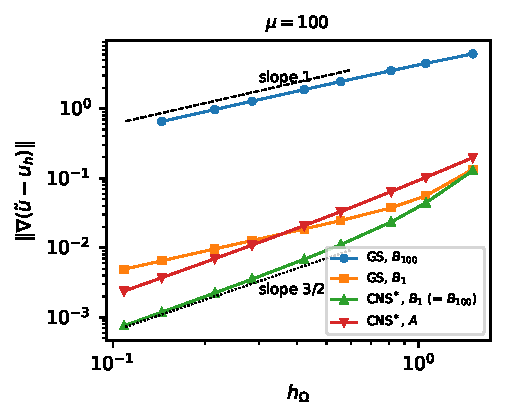
\includegraphics[width=0.48\textwidth]{figures/h1_rates.pdf}\hfill
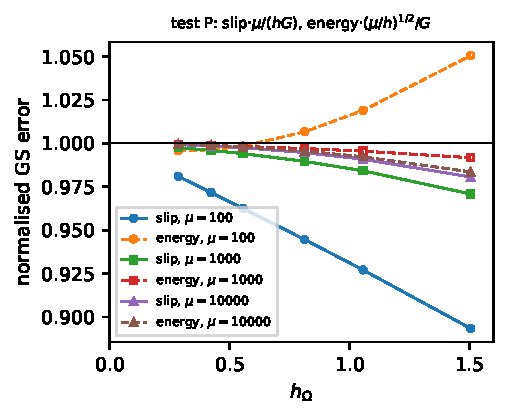
\includegraphics[width=0.48\textwidth]{figures/leading_term.pdf}
\caption{Left: $H^1$ errors at $\mu=100$. Once $G>0$, $\GS$ eventually has slope $1$, while $\CNS$ tends to slope $\frac32$ independently of the pressure. Right: the normalised slip and energy errors of $\GS$ on test P approach $1$ (Corollary~\ref{cor:Bp}).}
\label{fig:rates}
\end{figure}

\subsection{Pressure errors}
The pressure errors follow Section~\ref{sec:further} (Tables~\ref{tab:B100} and~\ref{tab:pB1}). For $\CNS$ the pressure error does not depend on the pressure data (for B$_1$, B$_{100}$ and C it agrees to $10^{-6}$ at $N=16$ and $3\cdot10^{-11}$ at $N=96$), and its $L^2$ rate decreases towards $\frac32$. For $\GS$ with $G>0$ the $L^2$ rate decreases towards $\frac12$; the first layer of triangles carries rate $0.48$--$0.50$ and the rest rate $0.9$--$1.0$, and the $L^\infty$ error on the first layer does not converge ($0.78$ for B$_1$, $77$ for B$_{100}$). On test P the first-layer pressure error of $\GS$ is $0.0958$ and $0.0793$ at $N=64$ and $96$, against $0.0961$ and $0.0796$ for the explicit first-layer field predicted by the theory. With $G=0$ (test A), $\GS$ behaves like $\CNS$.

\begin{table}[t]
\centering\small
\caption{$L^2$ pressure error $\norm{p^\circ-p_h}$, $\mu=100$. The ``off layer'' column is the $\GS$ error outside the first row of triangles, with the optimal constant removed.}\label{tab:pB1}
\begin{tabular}{rcccccc|cccc}
\toprule
 & \multicolumn{6}{c|}{test B$_1$ ($G>0$)} & \multicolumn{4}{c}{test A ($G=0$)}\\
$N$ & $\GS$ & rate & off layer & rate & $\CNS$ & rate & $\GS$ & rate & $\CNS$ & rate\\
\midrule
16 & $0.530$ & -- & $0.500$ & -- & $0.497$ & -- & $0.205$ & -- & $0.378$ & --\\
32 & $0.180$ & 1.22 & $0.121$ & 1.84 & $0.0767$ & 3.03 & $0.0648$ & 1.85 & $0.121$ & 1.81\\
48 & $0.137$ & 0.72 & $0.0805$ & 1.08 & $0.0287$ & 2.59 & $0.0329$ & 1.79 & $0.0623$ & 1.75\\
64 & $0.115$ & 0.61 & $0.0632$ & 0.88 & $0.0162$ & 2.08 & $0.0204$ & 1.73 & $0.0392$ & 1.69\\
96 & $0.0913$ & 0.60 & $0.0445$ & 0.89 & $0.00801$ & 1.80 & $0.0106$ & 1.68 & $0.0205$ & 1.65\\
\bottomrule
\end{tabular}
\end{table}

\subsection{The leak law and its constants}
Test P isolates the traction response exactly. Table~\ref{tab:P} and Figure~\ref{fig:rates} (right) show that the normalised slip and energy errors approach $1$, as Corollary~\ref{cor:Bp} predicts: at $N=96$ the energy ratios are within $0.5\%$ of $1$ for every $\mu$, and the defect of the slip ratio shrinks with $h/\mu$ ($0.019$, $0.0025$, $0.0007$ for $\mu=10^2,10^3,10^4$). Figure~\ref{fig:leak} shows the leak itself: at $N=32$, $\mu=100$, the normal trace of $u_h$ matches $(h/\mu)(p-\pbar)$ with relative $L^2(\Gh)$ misfit $0.055$, and the tangential trace is small and oscillates on the element scale. On test B$_1$ at $N=256$, $\GS$ itself gives slip and energy ratios $0.995$ and $1.001$.

The $H^1$ constant approaches the value $K=2.7565$ of Section~\ref{sec:leakflow} from both sides (Table~\ref{tab:hc}): from below at $\mu=100$, and from above at large $\mu$, where the excess is an element-scale oscillation nearly orthogonal to $U$ ($K_h^2\approx K^2(1+d_h^2)$; for example $2.7565\sqrt{1+0.175^2}=2.798$ against $2.796$ at $N=96$, $\mu=10^8$). The same slip and energy constants, and $H^1$ constants close to $K$, are observed for $k=5,6$ and on Clough--Tocher refinements with $k=2,3$ (Table~\ref{tab:Pv3}); for these elements the agreement with $K$ is observed, not proved.

\begin{table}[t]
\centering\small
\caption{The leading term of Corollary~\ref{cor:Bp}: normalised $\GS$ error on test P ($G=1.658$), $e=\ut-u_h$.}\label{tab:P}
\begin{tabular}{rrccc}
\toprule
$N$ & $\mu$ & $\norm{\nabla e}\,\mu/(hG)$ & $\norm{e}_{\Gh}\,\mu/(hG)$ & $\tnorm{e}(\mu/h)^{1/2}/G$\\
\midrule
16 & 100 & 2.464 & 0.893 & 1.050\\
32 & 100 & 2.612 & 0.945 & 1.007\\
64 & 100 & 2.684 & 0.972 & 0.996\\
96 & 100 & 2.708 & 0.981 & 0.996\\
96 & 1000 & 2.770 & 0.998 & 0.999\\
96 & 10000 & 2.790 & 0.9993 & 0.9994\\
\bottomrule
\end{tabular}
\end{table}

\begin{table}[t]
\centering\small
\caption{Approach to the $H^1$ constant $K=2.7565157$ (Theorem~\ref{thm:hc}) on test P: normalised $H^1$ error $K_h$ and relative $H^1$ distance $d_h$ between $(\mu/h)(\ut-u_h)$ and the leak flow, computed pointwise against the series solution.}\label{tab:hc}
\begin{tabular}{r|cc|cc|cc|cc}
\toprule
 & \multicolumn{2}{c|}{$\mu=10^2$} & \multicolumn{2}{c|}{$\mu=10^3$} & \multicolumn{2}{c|}{$\mu=10^4$} & \multicolumn{2}{c}{$\mu=10^8$}\\
$N$ & $K_h$ & $d_h$ & $K_h$ & $d_h$ & $K_h$ & $d_h$ & $K_h$ & $d_h$\\
\midrule
16 & 2.4642 & 0.193 & 2.7844 & 0.318 & 3.0562 & 0.539 & 3.3254 & 0.717\\
32 & 2.6117 & 0.124 & 2.7880 & 0.222 & 2.8751 & 0.323 & 2.9339 & 0.385\\
64 & 2.6843 & 0.084 & 2.7759 & 0.154 & 2.8082 & 0.206 & 2.8208 & 0.226\\
96 & 2.7084 & 0.067 & 2.7701 & 0.124 & 2.7899 & 0.163 & 2.7959 & 0.175\\
\bottomrule
\end{tabular}
\end{table}

\begin{figure}[t]
\centering
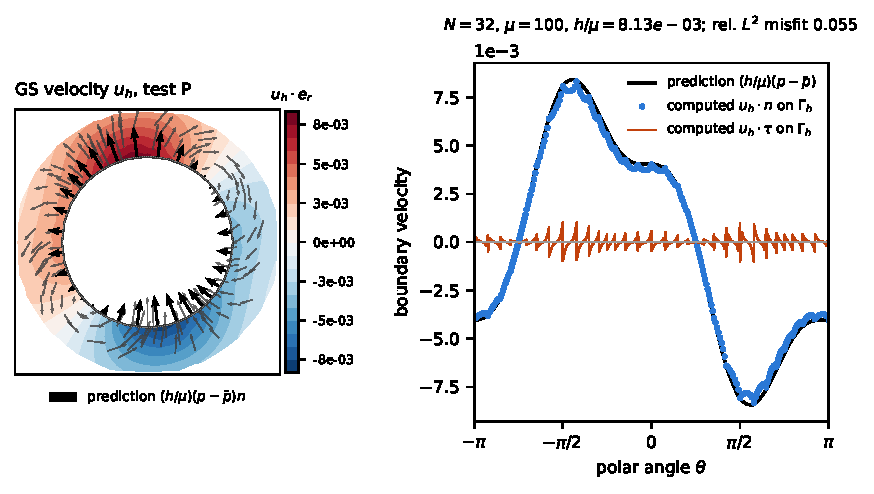
\includegraphics[width=\textwidth]{figures/leak_field.pdf}
\caption{The leak of the printed method on test P ($u=0$, so $u_h=-(\ut-u_h)$), $N=32$, $\mu=100$. Left: radial velocity $u_h\cdot e_r$ near the wall (colour) and $u_h$ (thin arrows); thick arrows show the prediction $(h/\mu)(p-\pbar)n$ at the chord midpoints. Right: normal and tangential traces of $u_h$ along $\Gh$ against $(h/\mu)(p-\pbar)$.}
\label{fig:leak}
\end{figure}

\begin{table}[t]
\centering\small
\caption{Normalised $\GS$ error on test P for other elements, at the finest level run.}\label{tab:Pv3}
\begin{tabular}{lrrccc}
\toprule
element & $\mu$ & $N$ & $\norm{\nabla e}\,\mu/(hG)$ & $\norm{e}_{\Gh}\,\mu/(hG)$ & $\tnorm{e}(\mu/h)^{1/2}/G$\\
\midrule
$k=5$ & 1000 & 128 & 2.768 & 0.9983 & 0.9994\\
$k=6$ & 1000 & 96 & 2.769 & 0.9976 & 0.9993\\
Clough--Tocher, $k=2$ & 1000 & 128 & 2.751 & 0.9982 & 0.9992\\
Clough--Tocher, $k=3$ & 1000 & 128 & 2.763 & 0.9983 & 0.9996\\
\bottomrule
\end{tabular}
\end{table}

\emph{Incompressibility is what saves the rate.} We computed exact discrete dual norms of the functionals used in the proofs, by saddle-point solves with the pointwise divergence constraint (Table~\ref{tab:lemma}). The dual norm of $v\mapsto\ip{S}{\dn v}$ with $S$ normal stays bounded on $\Zh$, but grows like $\hG^{-1/2}$ on $\VR$, and also on $\Zh$ for tangential $S$: exactly the dichotomy of Lemma~\ref{lem:cancel}. The transposed-gradient functional decays at rate $1.56$--$1.57$, confirming that the rate $\frac32$ of Lemma~\ref{lem:transposed} is sharp.

\begin{table}[t]
\centering\small
\caption{Exact discrete dual norms; rate in $\hG$ between $N=48$ and $N=64$ (positive means decay).}\label{tab:lemma}
\begin{tabular}{llc}
\toprule
functional & space & rate\\
\midrule
$\ip{S}{\dn v}$, $S$ normal & $\Zh$ & $+0.05$ (bounded, $\approx1.75$)\\
$\ip{S}{\dn v}$, $S$ normal & $\VR$ & $-0.52$\\
$\ip{S}{\dn v}$, $S$ tangential & $\Zh$ & $-0.52$\\
$\ip{(\nabla\ut)^{\mathsf T}n}{v}$, tests A / B & $\VR$ & $1.57$ / $1.56$\\
\bottomrule
\end{tabular}
\end{table}

\subsection{The penalty study}
The coercivity threshold $\mu^\ast$ on $\Zh$ is located by bisection on the inertia of the (unpivoted symmetric factorisation of the) velocity block augmented by a large multiple of the divergence penalty. Table~\ref{tab:thresh} and Figure~\ref{fig:thresh} give the results. Under refinement at fixed $h/\hG$, $\gamma^\ast$ increases by $3.4$, $1.8$ and $0.95$ per doubling, approaching the periodic-cell value $\gamma^\ast_\infty\approx21.4$ of Section~\ref{sec:penalty}. When the far field is coarsened with the wall fixed (part (b)), $\mu^\ast$ is linear in $h/\hG$ over more than a decade with slope $18$--$20$: the threshold is set locally at the wall, and the global normalisation of the penalty turns it into a $\rho$-scaling. For higher degree and on Clough--Tocher refinements the threshold is larger (Table~\ref{tab:threshv3}); in particular $\mu=100$ is \emph{below} the threshold for $k=5$ ($N\ge32$), $k=6$ and Clough--Tocher $k=3$, and our runs for those elements use $\mu=300$ and $1000$.

\begin{table}[t]
\centering\small
\caption{Coercivity threshold $\mu^\ast$ and $\gamma^\ast=\mu^\ast\hG/h$ ($k=4$).}\label{tab:thresh}
\textit{(a) Refinement at fixed $h/\hG\approx3.3$.}\\[2pt]
\begin{tabular}{lcccccccc}
\toprule
$N$ & 8 & 12 & 16 & 20 & 24 & 32 & 48 & 64\\
\midrule
$\rho$ & 3.41 & 4.16 & 4.70 & 5.08 & 5.36 & 5.73 & 6.13 & 6.35\\
$\mu^\ast$ & 50.3 & 51.8 & 59.3 & 60.3 & 63.3 & 66.0 & 69.1 & 70.7\\
$\gamma^\ast$ & 14.7 & 17.1 & 18.1 & 19.1 & 19.2 & 19.9 & 20.5 & 20.8\\
\bottomrule
\end{tabular}\par\vspace{6pt}
\textit{(b) Varying $h/\hG$ through the outer box $(-L,L)^2$.}\\[2pt]
\begin{tabular}{llccccc}
\toprule
 & $L$ & 2.5 & 5 & 10 & 20 & 40\\
\midrule
$N=16$ & $h/\hG$ & 3.28 & 5.90 & 11.3 & 22.2 & 43.9\\
 & $\mu^\ast$ & 59.3 & 112.1 & 208.0 & 411.5 & 809.3\\
\midrule
$N=32$ & $h/\hG$ & 3.33 & 5.79 & 10.8 & 21.1 & 41.5\\
 & $\mu^\ast$ & 66.0 & 113.9 & 218.0 & 422.2 & 835.7\\
\bottomrule
\end{tabular}
\end{table}

\begin{figure}[t]
\centering
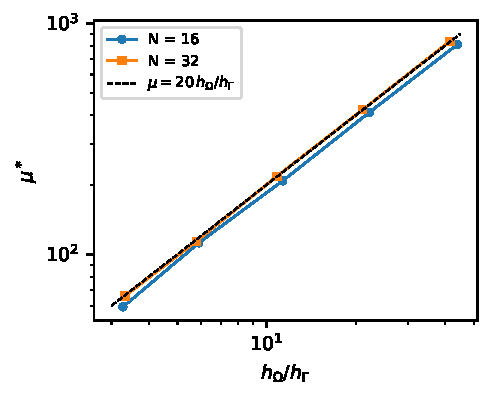
\includegraphics[width=0.55\textwidth]{figures/threshold.pdf}
\caption{Coercivity threshold $\mu^\ast$ against $h/\hG$ (Table~\ref{tab:thresh}(b)).}
\label{fig:thresh}
\end{figure}

\begin{table}[t]
\centering\small
\caption{Coercivity threshold $\gamma^\ast$ for higher degree and on Clough--Tocher (CT) refinements.}\label{tab:threshv3}
\begin{tabular}{lccccc}
\toprule
 & $N=8$ & $16$ & $32$ & $64$ & $128$\\
\midrule
$k=4$ & 14.7 & 18.1 & 19.9 & 20.8 & --\\
$k=5$ & 25.7 & 30.3 & 32.1 & 33.0 & --\\
$k=6$ & -- & 45.2 & 47.4 & 48.3 & --\\
CT, $k=2$ & 5.7 & 9.1 & 10.5 & 11.2 & 11.5\\
CT, $k=3$ & -- & 31.6 & 33.9 & 34.6 & --\\
\bottomrule
\end{tabular}
\end{table}

\emph{A growing penalty.} With $\mu=c(h_{16}/h)^\alpha$, $h_{16}=1.505$, the rates follow the predictions of Section~\ref{sec:growing} (Table~\ref{tab:rescue}). On test P, where only the leak is present, they are exactly $1+\alpha$ ($H^1$) and $(1+\alpha)/2$ (energy). On B$_1$ the $H^1$ rate of $\GS$ moves from $0.96$ to $1.42$--$1.52$ and the error at $N=96$ halves; on B$_1$ with $\alpha=\frac12$, $c=1000$ the measured energy rate $1.28$ is the geometric branch $(3-\alpha)/2$, the leak branch taking over only later.

\begin{table}[t]
\centering\small
\caption{$\GS$ (and $\CNS$) with $\mu=c(h_{16}/h)^\alpha$: rates between $N=64$ and $N=96$, and the asymptotic rates predicted in Section~\ref{sec:growing} (on test P, where only the leak is present, $1+\alpha$ and $(1+\alpha)/2$).}\label{tab:rescue}
\begin{tabular}{llccccc}
\toprule
test & method & $(\alpha,c)$ & $\norm{\nabla e}$ at $N=96$ & $H^1$ rate & energy rate & predicted\\
\midrule
P & $\GS$ & $(0,100)$ & $1.28\cdot10^{-2}$ & 0.95 & 0.49 & 1, 0.5\\
P & $\GS$ & $(\frac12,100)$ & $5.64\cdot10^{-3}$ & 1.45 & 0.73 & 1.5, 0.75\\
P & $\GS$ & $(1,100)$ & $2.47\cdot10^{-3}$ & 1.94 & 0.97 & 2, 1\\
B$_1$ & $\GS$ & $(0,100)$ & $1.27\cdot10^{-2}$ & 0.96 & 0.56 & 1, 0.5\\
B$_1$ & $\GS$ & $(\frac12,1000)$ & $5.81\cdot10^{-3}$ & 1.52 & 1.28 & 1.5, 0.75\\
B$_1$ & $\GS$ & $(1,100)$ & $5.03\cdot10^{-3}$ & 1.47 & 1.06 & 1.5, 1\\
B$_1$ & $\CNS$ & $(0,100)$ & $3.54\cdot10^{-3}$ & 1.64 & 1.53 & 1.5, 1.5\\
B$_1$ & $\CNS$ & $(1,100)$ & $5.21\cdot10^{-3}$ & 1.45 & 1.16 & 1.5, 1\\
A & $\GS$ & $(1,100)$ & $1.48\cdot10^{-2}$ & 1.34 & 1.16 & 1.5, 1\\
\bottomrule
\end{tabular}
\end{table} On test A ($G=0$) a growing penalty only costs: the $H^1$ constant moves towards that of the Dirichlet limit, $2.5$ times larger, and the energy error grows like $\gamma^{1/2}\hG^{3/2}$.

\emph{Flux correction.} Test F uses $\psi=(r^2-1)^3\sin(2x+1)\cos(\frac32y+\frac7{10})/400$ and $p=x^2y-y+x/2$: the cube makes $W\equiv0$, so the geometric slip $\norm{\ut}_{\Gh}$ is small, and the phase shifts break the symmetries, so the outer flux $m_R$ is nonzero (it decays like $h^{6.6}$). Every $z\in\Wh$ satisfies $\tnorm{\ut-z}\ge(\mu/h)^{1/2}|m_R|/|\Gh|^{1/2}$, a floor with constant exactly $1$. Table~\ref{tab:flux} shows the floor and its removal by the correction of Definition~\ref{def:flux}. Without correction the slip error of $\CNS$ is $(|m_R|^2/|\Gh|+\norm{\ut}^2_{\Gh})^{1/2}$ to three digits; with it, the slip error is $\norm{\ut}_{\Gh}$ to five digits. The $H^1$ errors with and without correction agree to relative $3\cdot10^{-6}$ ($N=16$) down to $10^{-9}$ ($N=64$), as Theorem~\ref{thm:unif} predicts.

\begin{table}[t]
\centering\small
\caption{Test F, $\CNS$ with uncorrected ($\gI$) and flux-corrected ($\tilde g_I$) outer data. Slip errors at $\mu=10^6$; energy errors at $\mu=10^8$, with the floor $(\mu/h)^{1/2}|m_R|/|\Gh|^{1/2}$.}\label{tab:flux}
\setlength{\tabcolsep}{3pt}
\begin{tabular}{rcccccccc}
\toprule
$N$ & $m_R$ & $\frac{|m_R|}{|\Gh|^{1/2}}$ & $\norm{\ut}_{\Gh}$ & slip, $\gI$ & slip, $\tilde g_I$ & $\tnorm e$, $\gI$ & $\tnorm e$, $\tilde g_I$ & floor\\
\midrule
16 & $2.04\cdot10^{-3}$ & $8.19\cdot10^{-4}$ & $2.40\cdot10^{-5}$ & $8.204\cdot10^{-4}$ & $2.396\cdot10^{-5}$ & 6.752 & 0.955 & 6.672\\
32 & $2.56\cdot10^{-5}$ & $1.02\cdot10^{-5}$ & $1.70\cdot10^{-6}$ & $1.038\cdot10^{-5}$ & $1.697\cdot10^{-6}$ & 0.187 & 0.149 & 0.114\\
64 & $3.75\cdot10^{-7}$ & $1.50\cdot10^{-7}$ & $1.09\cdot10^{-7}$ & $1.851\cdot10^{-7}$ & $1.091\cdot10^{-7}$ & 0.0123 & 0.0121 & 0.0023\\
\bottomrule
\end{tabular}
\end{table}

\emph{Higher degree and Clough--Tocher refinements.} Table~\ref{tab:ratesv3} gives $H^1$ rates at the finest pair of levels for $k=5,6$ and for Clough--Tocher refinements. $\CNS$ tends to rate $\frac32$ for $k=5,6$; $\GS$ tends to rate $1$ once $G>0$ (for $k=5$, $\mu=300$, its rate on B$_1$ decreases monotonically, $1.63,1.58,1.48,1.38,1.28,1.20$ for $N=24,\dots,128$), and the leak part $D:=u_{\GS}-u_{\CNS}$ already has rate $1.03$--$1.15$ and normalised slip and energy ratios within $1.5\%$ of $1$. At $\mu=1000$ the crossover of $\GS$ comes later, exactly as for $k=4$.

\begin{table}[t]
\centering\small
\caption{$H^1$ rates at the finest pair of levels (energy rate of $\CNS$ in parentheses); $D=u_{\GS}-u_{\CNS}$ is the leak part.}\label{tab:ratesv3}
\begin{tabular}{llrrccc}
\toprule
element & test & $\mu$ & $N$ & $\GS$ & $\CNS$ & $D$\\
\midrule
$k=5$ & B$_1$ & 300 & $96\to128$ & 1.20 & 1.59 (1.53) & 1.03\\
$k=5$ & B$_1$ & 1000 & $96\to128$ & 1.53 & 1.58 (1.54) & 1.13\\
$k=6$ & B$_1$ & 300 & $64\to96$ & 1.27 & 1.61 (1.54) & 1.04\\
$k=6$ & B$_1$ & 1000 & $64\to96$ & 1.57 & 1.61 (1.54) & 1.15\\
CT, $k=3$ & A & 1000 & $96\to128$ & 1.56 & 1.56 (1.55) & --\\
CT, $k=2$ & B$_1$ & 100 & $192\to256$ & 1.91 & 1.91 (1.91) & 1.01\\
\bottomrule
\end{tabular}
\end{table}

\subsection{Strong imposition and the \texorpdfstring{$h^{1/2}$}{h^(1/2)} phenomenon}\label{sec:num:strong}
Table~\ref{tab:strong} compares strongly imposed no-slip ($u_h=0$ at every node of $\Gh$, no Nitsche terms, same element) with $\GS$ and $\CNS$ on test A.
\begin{itemize}
\item On mesh (a) the first-layer diagonals alternate, so every other polygon vertex lies in only two triangles. The $H^1$ rate of strong imposition falls towards $\frac12$ ($0.56$ at $N=128$); the largest vertex-gradient error tends to $1.99$, which is $|\dn u\cdot\tau|=2$ for this flow: the discrete gradient vanishes at the locked vertices, and the pressure grows like $h^{-1/2}$ although $p\equiv0$. The counting lower bound of Theorem~\ref{thm:st:count} is within a factor $3.0$--$3.15$ of the measured error.
\item On mesh (s) every polygon vertex lies in three triangles, and strong imposition converges with rates $1.93\to1.61$, like the Nitsche methods, with an error about $2.5$ times larger. The slow drift of the rate (to $1.547$ at $N=192$) is a relative $O(\hG)$ correction: the data fit $E\approx a\hG^{3/2}(1+\beta\hG)$ with $\beta\approx1.1$--$1.3$. The vertex-gradient error decays like $h$, exactly as Lemma~\ref{lem:st:local}(d) predicts. Imposing $u_h=\ut$ instead of $0$ at the nodes of $\Gh$ gives rate about $4$: the whole defect is the transfer of the no-slip value from $\Gamma$ to $\Gh$.
\item $\GS$ and $\CNS$ do not see the change of mesh: at every $N\le128$ their errors on meshes (a) and (s) differ by at most $6\%$.
\item With a single locked vertex the strong-imposition rate falls to $1$ ($1.06$ at $N=128$), the raw pressure error does not converge, and the filtered pressure of Theorem~\ref{thm:st:locks}(d) converges at the velocity rate. With needles at the wall of angle $\varepsilon=0.3,\hG,\hG^2$ the rates approach $\frac32$, $1$, $\frac12$ as predicted, although the last two limits are not yet reached at $N\le96$.
\end{itemize}

\begin{table}[t]
\centering\small
\caption{Strong imposition against Nitsche: $H^1$ error, test A, $k=4$, $\mu=100$. Mesh (s): every polygon vertex in three triangles; mesh (a): alternating first-layer diagonals (vertices in two or four triangles).}\label{tab:strong}
\begin{tabular}{rrrrrrrrr}
\toprule
$N$ & \multicolumn{2}{c}{strong, (a)} & \multicolumn{2}{c}{strong, (s)} & \multicolumn{2}{c}{$\GS$, (s)} & \multicolumn{2}{c}{$\CNS$, (s)}\\
\cmidrule(lr){2-3} \cmidrule(lr){4-5} \cmidrule(lr){6-7} \cmidrule(lr){8-9}
 & error & rate & error & rate & error & rate & error & rate\\
\midrule
16 & $9.03\cdot10^{-1}$ & -- & $4.62\cdot10^{-1}$ & -- & $1.72\cdot10^{-1}$ & -- & $1.98\cdot10^{-1}$ & --\\
32 & $5.72\cdot10^{-1}$ & 0.72 & $1.43\cdot10^{-1}$ & 1.86 & $5.55\cdot10^{-2}$ & 1.79 & $6.41\cdot10^{-2}$ & 1.80\\
64 & $3.75\cdot10^{-1}$ & 0.62 & $4.56\cdot10^{-2}$ & 1.71 & $1.81\cdot10^{-2}$ & 1.68 & $2.08\cdot10^{-2}$ & 1.69\\
96 & $2.98\cdot10^{-1}$ & 0.59 & $2.38\cdot10^{-2}$ & 1.65 & $9.57\cdot10^{-3}$ & 1.63 & $1.09\cdot10^{-2}$ & 1.64\\
128 & $2.54\cdot10^{-1}$ & 0.56 & $1.52\cdot10^{-2}$ & 1.61 & $6.11\cdot10^{-3}$ & 1.59 & $6.96\cdot10^{-3}$ & 1.60\\
\bottomrule
\end{tabular}
\end{table}

\subsection{Caveats}
Three limitations should be kept in mind. First, the production penalty $\mu=100$ is close to the stability thresholds, as discussed above, so the measured constants are partly pre-asymptotic. Second, the manufactured solutions are smooth up to the corners of the box; for data-driven problems the corner singularities of the box would limit the bulk term (Assumption~\ref{ass:D}), though not the wall term that is the subject of this paper. Third, on Clough--Tocher refinements with $k=2,3$ the test pressure is not in the pressure space, and the pressure-independence of $\CNS$ holds only up to a term of order $h^{k+1/2}$ that scales with the amplitude of $p$; on test B$_1$ the rate $\frac32$ is not yet visible there, because the interpolation error of the steep velocity dominates \cite{PadhiExt}.
